\chapter{Expressive Speech synthesis}

%This chapter explain how the project was carried out
%In this chapter of the document, the development process that has been followed in order to complete this project is explained.

\section{Baseline development}

The first stage of this project was to develop a baseline speech synthesizer. This model is used as a reference when comparing the results of the subsequent experiments explained in later sections of this chapter. The architecture is based on the work done by \cite{santi06} by using the Socrates Text-to-speech framework, which is based on the Keras deep learning library. This is a RNN-LSTM based model, which, as mentioned in section \ref{sec:rnn-tts}, contains a duration model and an acoustic model which are trained independently.

\begin{figure}[h]
    \centering
    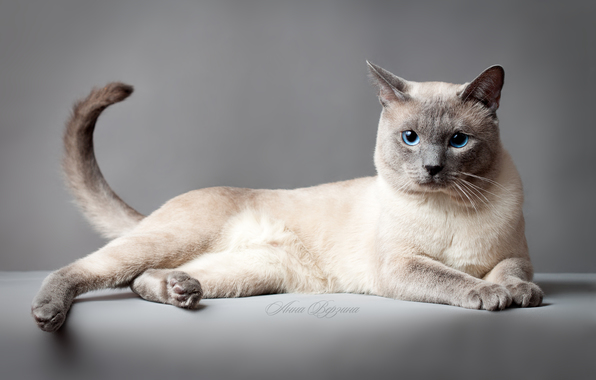
\includegraphics[width=8cm]{figures/cat}
    \caption{Baseline model}
    \label{fig:lstm-tts}
\end{figure}

\begin{itemize}
    \item The duration model predicts the duration of a phoneme. This model takes a vector of linguistic features with information about the phoneme and its context and outputs a single value that is the log-compressed duration of the phoneme (this log-compression is explained in the data preparation section).
    \item The acoustic model predicts the excitation and spectral parameters of a frame of speech. The input of this system is the same vector of linguistic features, the normalized duration of the predicted value from the pervious model and the relative duration of the frame within the duration of the phoneme. The output of this model is also explained in the next section.
\end{itemize}

%The overall system, without going in depth in the system is the one shown in Figure \ref{fig:sys}, where a set of acoustic features are produced from the audio streams and another set of linguistic features are obtained from the transcriptions.

%In the following subsections we go in more detail into each of the shown modules from Figure \ref{fig:sys}. The explanations are not a special case of the baseline system but they are also relevant for the final system with the added expressiveness features from the other sections of this chapter.
%The following sections explain how the data that is used to train this architecture is obtained from our speech corpus.

\subsection{Data preparation}

%The developed speech synthesizer is an RNN-based architecture similar to the one presented in chapter 2. As mentioned in that section, the architecture from the baseline system is composed of two sections: a duration model and an acoustic model. It is important to note that this system does not produce the output waveform directly but instead it produces spectral and excitation coefficients like in SPSS based systems. This means that the speech database that we use will have to be processed in order to train the system.

The database that has been used for this project contains approximately 20 hours or several audiobooks along with the transcriptions. The data came from the Blizzar challenge \cite{blizzard} and is already segmented at the utterance level, removing the need to align the whole audio stream with the raw text data. The reason we chose this database was because of its richness in expressive content. Table \ref{tab:blizard} shows some information about the audio files that we had.

% table with audio information (Sampling, bit depth, channels, etc...)
\begin{table}[h]
    \centering
    \begin{tabular}{l|c}
        Metric & Value \\
        \hline
        Sampling rate ($Hz$) & 16000 \\
        Bit depth (bits) & 16 \\
        Channels & mono \\
        Length (seconds mean) & 7.23 \\
        Length (seconds std) & 4.52 \\
        Speakers & 1
    \end{tabular}
    \caption{Information about the Blizzard Challenge utterances.}
    \label{tab:blizard}
\end{table}

%Every speech waveform is decoded at a frame level by using a vocoder using a sliding window that advances 25 milliseconds between consecutive windows. The vocoder that we used for this project is Ahocoder, an Harmonics plus Noise Model that is described in detail at \cite{vocoder_ah}. In Figure \ref{fig:wav-prep} it is shown how each utterance is processed.

\subsection{Obtaining Acoustic features}

As mentiones in secton \ref{sec:rnn-tts}, this RNN based speech synthesizer is a SPSS case and as such it doesn't output the waveforms directly but the excitation and spectral parameters before they are reconstructed by a vocoder. The vocoder that we used is Ahocoder \cite{vocoder_ah}.

Every audio file is framed by means of a sliding window with a stride of 25 milliseconds. Ahocoder then processes each frame to produce a set of excitation and spectral parameters which are:

\begin{itemize}
    \item{Mel Frequency Cepstral Coefficients (MFCC) of order $p = 39$, which corresponds to $40$ coefficients.}
    \item{Pitch contour ($log(F_0)$). Unvoiced frames correspond to $F_0 = 0$ value of $-\inf$ after the logarithm. Ahocoder outputs a value of $-10^8$ when the frame is unvoiced.}
    \item{Maximum voiced frequency ($fv$), This value is 0 when a frame is unvoiced.}
    \item{Voiced/Unvoiced (UV) flag. This value indicates if a given frame of audio corresponds to a voiced or unvoiced sound and can be obtained using the $fv$ or $log(f0)$ outputs of Ahocoder.}
\end{itemize}

The data is not used as it is, at the output of the Ahocoder. These acoustic predictors are normalized before they are used to train the acoustic model for a good behavior of the back-propagation algorithm, as discussed in \cite{santi06}. The outputs of the Ahocoding process have been normalized so that they are bound between a minimum and a maximum value range. This range is choosen to be ${0.01, 0.99}$ for better convergence properties. The normalization of the acoustic outputs is shown in equation \ref{eq:out-norm}

\begin{equation}
    y = 0.01 + (0.99 - 0.01) \frac{y - y_{min}}{y_{max} - y_{min}}
    \label{eq:out-norm}
\end{equation}

This doesn't work for the $log(F_0)$ and $f_v$ features since their high dynamic range will compress the values from the viced frames too much. \cite{santi06} solves it by keeping the values from the voiced frames and interpolating the values in the unvoiced regions as shown in Equation \ref{eq:linear-f0}:

\begin{equation}
    log F_0^i = log F_0^p + (log F_0^n - log F_0^p) \cdot \frac{i-p}{n-p}
    \label{eq:linear-f0}
\end{equation}

Where $n$ is the next voiced frame's frame index, $F_0^n$ is the next voiced frame's first value, p is the previous voiced value's frame index, $F_0^p$ is the previous voiced value and $F_0^i$ is the $i$-th new interpolated value to be replaced in the original output of the Ahocoding process (Figure \ref{fig:f0-int} has an example of this interpolation). We can then use the UV flag to recover the original format after denormalization and reconstruct the waveform.

\begin{figure}
    \centering
    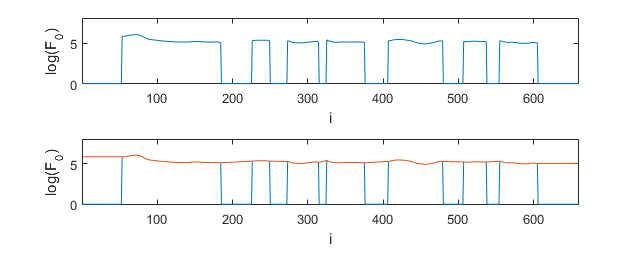
\includegraphics[width=12cm]{figures/f0.png}
    \caption{$F_0$ contour interpolation}
    \label{fig:f0-int}
\end{figure}

%The audio transcriptions have to be segmented at phoneme level into the linguistic features of th system. This is done using both the audio and the transcriptions in a process called forced-alignment to obtain a prediction of the duration of each phoneme uttered in each sentence. This process and the linguistic features that come out of this process are explained in the following section:

These acoustic features are used to train the acoustic model of the system. The data is structured for training as a series of input-output vector pairs layed out in the following manner in the training data tables:

\begin{figure}[h]
\begin{lstlisting}
<linguistic features 1, duration 1> <acoustic features 1>
<linguistic features 1, duration 1> <acoustic features 2>
<linguistic features 1, duration 1> <acoustic features 3>
<linguistic features 2, duration 2> <acoustic features 4>
<linguistic features 2, duration 2> <acoustic features 5>
<linguistic features 2, duration 2> <acoustic features 6>
<linguistic features 2, duration 2> <acoustic features 7>
<linguistic features 3, duration 3> <acoustic features 8>
<linguistic features 3, duration 3> <acoustic features 9>
...
\end{lstlisting}
\caption{Training table used to train the acoustic model is stored in the server disk.}
\end{figure}

Which are the examples that are used to train the acoustic model. Some of the inputs are repeated deppending on the duration of the phonemes. The linguistic features are explained in the next section. 

\subsection{Obtaining linguistic features}

Each of the audio transcriptions is transformed into a lower level phonetic representation called Label that contains a set of both real and categorical descriptors with information about each phoneme and its context within a sentence. Table \ref{tab:lab-format} contains a description of the values that are included in this representation.

When a phoneme is converted into a Label, it has the following format:

%TODO formato del lab de ogmios
\begin{lstlisting}
p1^p2$-$p3$+$p4$=$p5~p6_p7/A:a1_a2_a3/B:b1-b2-b3~b4-b5&b6-b7#b8-b9$b10...
-b11!b12-b13;b14-b15|b16/C:c1+c2+c3/D:d1_d2/E:e1+e2~e3+e4&e5+e6#e7+e8...
/F:f1_f2/G:g1_g2/H:h1=h2~h3=h4|h4/I:i1_i2/J:j1+j2-j3
\end{lstlisting}

\begin{longtable}[!htpb]{p{0.1\textwidth} p{0.9\textwidth}}
\toprule
\multicolumn{2}{c}{label format} \\
\cline{1-2}
Symbol    & Description \\
\midrule
p1      & phoneme identity before the previous phoneme \\
p2      & previous phoneme identity \\
p3      & current phoneme identity \\
p4		& next phoneme identity \\
p5		& the phoneme after the next phoneme identity \\
p6		& position of the current phoneme identity in the current syllable (forward) \\
p7		& position of the current phoneme identity in the current syllable (backward) \\
\midrule
a1 & whether the previous syllable is stressed or not (0; not, 1: yes)\\
a2 & whether the previous syllable is accented or not (0; not, 1: yes)\\
\caption*{\tablename{} \ref{table:lab_format} (continued)}\\
\toprule
a3 & number of phonemes in the previous syllable \\
b1 & whether the current syllable stressed or not (0: not, 1: yes)\\
b2 & whether the current syllable accented or not (0: not, 1: yes)\\
b3 & the number of phonemes in the current syllable\\
b4 & position of the current syllable in the current word (forward)\\
b5 & position of the current syllable in the current word (backward)\\
b6 & position of the current syllable in the current phrase(forward)\\
b7 & position of the current syllable in the current phrase(backward)\\
b8 & number of stressed syllables before the current syllable in the current phrase\\
b9 & number of stressed syllables after the current syllable in the current phrase\\
b10 & number of accented syllables before the current syllable in the current phrase\\
b11 & number of accented syllables after the current syllable in the current phrase\\
b12 & number of syllables from the previous stressed syllable to the current syllable\\
b13 & number of syllables from the current syllable to the next stressed syllable\\
b14 & number of syllables from the previous accented syllable to the current syllable\\
b15 & number of syllables from the current syllable to the next accented syllable\\
b16 & name of the vowel of the current syllable\\
\midrule
c1 & whether the next syllable stressed or not (0: not, 1:yes) \\
c2 & whether the next syllable accented or not (0: not, 1:yes) \\
c3 & the number of phonemes in the next syllable \\
\midrule
d1 & gpos (guess part-of-speech) of the previous word \\
d2 & number of syllables in the previous word \\
\midrule
e1 & gpos (guess part-of-speech) of the current word \\
e2 & number of syllables in the current word \\
e3 & position of current word in the current phrase (forward) \\
e4 & position of current word in the current phrase (backward) \\
e5 & number of content words before the current word in the current phrase \\
e6 & number of content words after the current word in the current phrase \\
e7 & number of words from the previous content word to the current word \\
e8 & number of words from the current word to the next content word \\
\midrule
f1 & gpos (guess part-of-speech) of the next word \\
f2 & number of syllables in the previous word \\
\midrule
g1 & number of syllables in the previous phrase \\
g2 & number of words in the previous phrase \\
\midrule
h1 & number of syllables in the current phrase \\
\caption*{\tablename{} \ref{table:lab_format} (continued)}\\
\toprule
h2 & number of words in the current phrase \\
h3 & position of the current phrase in utterance (forward) \\
h4 & position of the current phrase in utterance (backward) \\
h5 & Phrase modality (question, exclamation, etc.)\\
\midrule
i1 & number of syllables in the next phrase \\
i2 & number of words in the previous phrase \\
\midrule
j1 & number of syllables in this utterance \\
j2 & number of words in this utterance \\
j3 & number of phrases in this utterance \\
\bottomrule
\caption{\label{table:lab_format}Context-dependent label format.}\\
\end{longtable}


A full example of this conversion is shown in \ref{fig:sentence-lab}:

\begin{figure}[h]
\begin{lstlisting}[basicstyle=\tiny,frame=single]
pau^D-i+O:=t~2_1/A:0_0_2/B:0-0-2~1-1&1-10#0-0$0-2!0-0;3-4|i/C:0+0+1/D:NN_2/E:DT+1~1+5&0+3#0+1/F:NN_6/G:3_2/H:10=5~3=1|F/I:0_0/J:10+16-2
D^i-O:+t=@~1_1/A:0_0_2/B:0-0-1~1-6&2-9#0-0$0-2!0-0;4-3|O:/C:0+0+2/D:DT_1/E:NN+6~2+4&0+3#1+1/F:IN_1/G:3_2/H:10=5~3=1|F/I:0_0/J:10+16-2
i^O:-t+@=b~1_2/A:0_0_1/B:0-0-2~2-5&3-8#0-0$0-2!0-0;5-2|@/C:0+0+2/D:DT_1/E:NN+6~2+4&0+3#1+1/F:IN_1/G:3_2/H:10=5~3=1|F/I:0_0/J:10+16-2
O:^t-@+b=aI~2_1/A:0_0_1/B:0-0-2~2-5&3-8#0-0$0-2!0-0;5-2|@/C:0+0+2/D:DT_1/E:NN+6~2+4&0+3#1+1/F:IN_1/G:3_2/H:10=5~3=1|F/I:0_0/J:10+16-2
t^@-b+aI=Q~1_2/A:0_0_2/B:0-0-2~3-4&4-7#0-0$0-2!0-0;6-1|aI/C:0+1+1/D:DT_1/E:NN+6~2+4&0+3#1+1/F:IN_1/G:3_2/H:10=5~3=1|F/I:0_0/J:10+16-2
@^b-aI+Q=g~2_1/A:0_0_2/B:0-0-2~3-4&4-7#0-0$0-2!0-0;6-1|aI/C:0+1+1/D:DT_1/E:NN+6~2+4&0+3#1+1/F:IN_1/G:3_2/H:10=5~3=1|F/I:0_0/J:10+16-2
b^aI-Q+g=r~1_1/A:0_0_2/B:0-1-1~4-3&5-6#0-0$0-1!0-0;7-5|Q/C:0+0+3/D:DT_1/E:NN+6~2+4&0+3#1+1/F:IN_1/G:3_2/H:10=5~3=1|F/I:0_0/J:10+16-2
aI^Q-g+r=@~1_3/A:0_1_1/B:0-0-3~5-2&6-5#0-0$1-1!0-0;1-4|@/C:0+0+2/D:DT_1/E:NN+6~2+4&0+3#1+1/F:IN_1/G:3_2/H:10=5~3=1|F/I:0_0/J:10+16-2
Q^g-r+@=f~2_2/A:0_1_1/B:0-0-3~5-2&6-5#0-0$1-1!0-0;1-4|@/C:0+0+2/D:DT_1/E:NN+6~2+4&0+3#1+1/F:IN_1/G:3_2/H:10=5~3=1|F/I:0_0/J:10+16-2
g^r-@+f=i~3_1/A:0_1_1/B:0-0-3~5-2&6-5#0-0$1-1!0-0;1-4|@/C:0+0+2/D:DT_1/E:NN+6~2+4&0+3#1+1/F:IN_1/G:3_2/H:10=5~3=1|F/I:0_0/J:10+16-2
r^@-f+i=@~1_2/A:0_0_3/B:0-0-2~6-1&7-4#0-0$1-1!0-0;2-3|i/C:0+0+2/D:DT_1/E:NN+6~2+4&0+3#1+1/F:IN_1/G:3_2/H:10=5~3=1|F/I:0_0/J:10+16-2
@^f-i+@=v~2_1/A:0_0_3/B:0-0-2~6-1&7-4#0-0$1-1!0-0;2-3|i/C:0+0+2/D:DT_1/E:NN+6~2+4&0+3#1+1/F:IN_1/G:3_2/H:10=5~3=1|F/I:0_0/J:10+16-2
f^i-@+v=@~1_2/A:0_0_2/B:0-0-2~1-1&8-3#0-0$1-1!0-0;3-2|@/C:0+0+1/D:NN_6/E:IN+1~3+3&1+2#1+2/F:DT_1/G:3_2/H:10=5~3=1|F/I:0_0/J:10+16-2
i^@-v+@=h~2_1/A:0_0_2/B:0-0-2~1-1&8-3#0-0$1-1!0-0;3-2|@/C:0+0+1/D:NN_6/E:IN+1~3+3&1+2#1+2/F:DT_1/G:3_2/H:10=5~3=1|F/I:0_0/J:10+16-2
@^v-@+h=O:~1_1/A:0_0_2/B:0-0-1~1-1&9-2#0-0$1-1!0-0;4-1|@/C:0+1+3/D:IN_1/E:DT+1~4+2&2+1#1+1/F:NN_1/G:3_2/H:10=5~3=1|F/I:0_0/J:10+16-2
v^@-h+O:=s~1_3/A:0_0_1/B:0-1-3~1-1&10-1#0-0$1-0!0-0;5-0|O:/C:0+0+0/D:DT_1/E:NN+1~5+1&2+1#2+0/F:SIL_0/G:3_2/H:10=5~3=1|F/I:0_0/J:10+16-2
@^h-O:+s=pau~2_2/A:0_0_1/B:0-1-3~1-1&10-1#0-0$1-0!0-0;5-0|O:/C:0+0+0/D:DT_1/E:NN+1~5+1&2+1#2+0/F:SIL_0/G:3_2/H:10=5~3=1|F/I:0_0/J:10+16-2
h^O:-s+pau=_~3_1/A:0_0_1/B:0-1-3~1-1&10-1#0-0$1-0!0-0;5-0|O:/C:0+0+0/D:DT_1/E:NN+1~5+1&2+1#2+0/F:SIL_0/G:3_2/H:10=5~3=1|F/I:0_0/J:10+16-2
O:^s-pau+_=_~1_1/A:0_1_3/B:0-0-1~1-1&0-11#0-0$0-2!0-0;1-0|_/C:0+0+0/D:NN_1/E:SIL+1~0+6&0+3#1+0/F:SIL_0/G:3_2/H:10=5~3=1|F/I:0_0/J:10+16-2
\end{lstlisting}
    \label{fig:sentence-lab}
    \caption{Label representation of the phrase "the autobiography of a horse."}
\end{figure}

%To convert the sentences to these Label representations, along with a prediction of the duration of each phoneme so we can use them as examples to train the synthesizer models, the Ogmios framework \cite{bonafonte2006ogmios} was used during the development of this project. In this program, a series of modules are combined in order to perform the task of phoneme segmntation and duration prediction. Figure \ref{fig:ogmios-pipeline} shows the Ogmios modules:

This label conversion is carried out with the aid of the Ogmios framework \cite{bonafonte2006ogmios}. This program offers a collection of speech processing modules that are combined to perform a given task. For the case of this project, it is used to obtain this label representation and to predict the duration of each of the phonemes in the sentences from the Blizzard corpus. Figure \ref{fig:ogmios-pipeline} shows the steps that it takes to obtain this information:

\tikzstyle{block} = [rectangle, draw, fill=blue!20, text width=6em, text centered, rounded corners, minimum height=4em]
\tikzstyle{red-block} = [ellipse, draw, fill=blue!20, text width=6em, text centered, rounded corners, minimum height=4em]
\tikzstyle{line} = [draw, -latex']

\begin{figure}[h]
    \centering
    \begin{tikzpicture}[node distance = 3cm, auto]
        \node[block] (bl0) {(1) Text normalization};
        \node[block, right of=bl0] (bl1) {(2) Phonetic transcription};
        \node[block, right of=bl1] (bl2) {(3) Context dependant HMMs};
        \node[block, right of=bl2] (bl3) {(4) Force alignment};
        \node[block, right of=bl3] (bl4) {(5) Label format};
        \path[line] (bl0) -- (bl1);
        \path[line] (bl1) -- (bl2);
        \path[line] (bl2) -- (bl3);
        \path[line] (bl3) -- (bl4);
    \end{tikzpicture}

    \caption{Ogmios modules used to predict phoneme duration.}
    \label{fig:ogmios-pipeline}
\end{figure}

\begin{enumerate}
    \item The text normalization module converts numeric values, dates, etc to its corresponding text form.
    \item The phonetic transcription module provides the pronunciation of the words.
    \item The HMM module estimates a left-to-right HMM model for each of the phonemes (Figure \ref{fig:hmm}) using the speech spectral parameters.
    %\item For each of the sentences it chains their phoneme HMMs and computes the most proabable sequence of states to predict the duration of each phoneme using the Bitervi algorithm.
    \item Given the phonemes of a sentence, it chains the HMM models and the most probable sequence of states is calculates using the Bitervi algorithm. With this information it can calculate the duration of each phoneme.
    \item The phonetic transcriptions along with the duration predictions are converts to the label format from table \ref{tab:lab-format}.
\end{enumerate}

This data also has to be normalized prior to training. The label format contains both categorical features and real features. The categorical information is encoded so that all categories are orthogonal to each other by using a one-hot encoding. As a small example of a one-hot encoding, consider the three categories $\{A, B, C\}$. Its one-hot encoding would be $\{(1,0,0), (0,1,0), (0,0,1)\}$.

The real fratures are normalized so that the mean equals zero and the standard deviation equals one. This is called z-norm and the operation is shown in \ref{eq:znorm}.

\begin{equation}
    z = \frac{x - \mu}{\sigma}
    \label{eq:znorm}
\end{equation}

As for the predicted duration of each phoneme, rather than using the raw value and as previously mentioned, it is log-compressed to avoid having a long-tailed distribution that can distort the training of the model when using the Mean Square Error (ME) minimization as discussed in \cite{santi06}. Figure \ref{fig:hist-d} contains the histogram of the raw predicted durations and the histogram after the log-compression operation.
%Instead of predicting the duration in milliseconds produced by Ogmios, we take the logarithm to avoid having a long tailed distribution that distorts the training using the Mean Square Error (MSE) minimization as discussed in \cite{santi06}. Figure \ref{fig:hist-d} contains the histogram of these values before and after the log operation.

\begin{figure}[h]
    \centering
    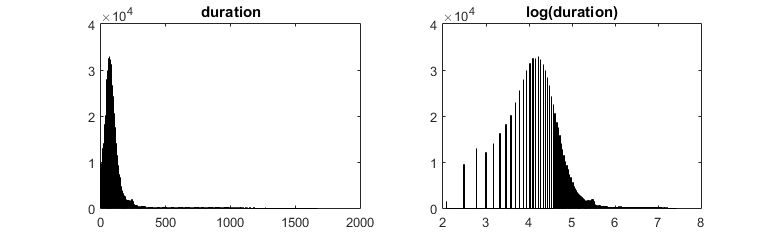
\includegraphics[width=14cm]{figures/dur}
    \caption{Histogram of the phoneme duration predictions by Ogmios.}
    \label{fig:hist-d}
\end{figure}

Once we have ensambled the linguistic features, we discard of those who reference the past and only keep the ones tagged with an asterisk ($*$). This is because the models are based on LSTM-RNN which are known to be good at modeling long term dependencies\cite{hochreiter1997long}.

\section{Expressive synthesis development}

%TODO
The baseline system has been explained. Once we had the system up and running it was time to introduce the modifications that would allow for expressive speech to be modeled by the system. The way this is done in this project is by introducing a new set of features as inputs to the system (both the duration and acoustic model). These are known as the embedding that encapsulate the information about the way a given sentence is supposed to be uttered as. In this section we describe the process of obtaining these new features. Other than these new inputs, the developed system shares the same architecture from the baseline system.

\subsection{Sentiment analysis \& embedding extraction task}

To obtain the embeddings, we define three 
%Explain the two networks, the datasets used and how the data was prepared to be fed into the training process and how to obtain the expressive embeddings that will be used in the next section

\section{Experiments}

Explain the experiments that were carried out and whose subsequent evaluation and results are presented in the next chapter
